\documentclass[
	a4paper,					% paper format
	10pt,							% fontsize
	twoside,					% double-sided
	openright,				% begin new chapter on right side
	notitlepage,			% use no standard title page
	parskip=half,			% set paragraph skip to half of a line
]{scrreprt}					% KOMA-script report

\raggedbottom
\KOMAoptions{cleardoublepage=plain}			% Add header and footer on blank pages
\usepackage[utf8]{inputenc}  							% Unix/Linux - load extended character set (ISO 8859-1)

\usepackage{csquotes}
\usepackage[hidelinks]{hyperref}
\usepackage{color}

% Code Segments
\usepackage{listings}

\usepackage[english]{babel}										% english hyphenation
%\usepackage[ansinew]{inputenc}  							% Windows - load extended character set (ISO 8859-1)
\usepackage{fancyhdr}													% simple manipulation of header and footer
\usepackage{etoolbox}													% color manipulation of header and footer
\usepackage{graphicx}                      		% integration of images
\usepackage{float}														% floating objects
\usepackage{caption}													% for captions of figures and tables
\usepackage{booktabs}													% package for nicer tables
\usepackage{tocvsec2}													% provides means of controlling the sectional numbering
\usepackage{tabularx}
%---------------------------------------------------------------------------

% Set up page dimension
%---------------------------------------------------------------------------
\usepackage{geometry}
\geometry{
	a4paper,
	left=28mm,
	right=15mm,
	top=30mm,
	headheight=20mm,
	headsep=10mm,
	textheight=242mm,
	footskip=15mm
}


% Compact Itemize:
%---------------------------------------------------------------------------
\newenvironment{compactitemize}
{ \begin{itemize}
    \setlength{\itemsep}{0pt}
    \setlength{\parskip}{0pt}
    \setlength{\parsep}{0pt}     }
{ \end{itemize}                  }
\newenvironment{compactenumerate}
{ \begin{enumerate}
    \setlength{\itemsep}{0pt}
    \setlength{\parskip}{0pt}
    \setlength{\parsep}{0pt}     }
{ \end{enumerate}  				 }

\RequirePackage{color}                          % Color (not xcolor!)
\definecolor{linkblue}{rgb}{0,0,0.8}            % Standard
\definecolor{darkblue}{rgb}{0,0.08,0.45}        % Dark blue
\definecolor{bfhgrey}{rgb}{0.41,0.49,0.57}      % BFH grey
\definecolor{linkcolor}{rgb}{0,0,0.8}  
\definecolor{darkblue}{rgb}{0,.2,.4}
\definecolor{darkgray}{rgb}{.4,.4,.4}
\definecolor{purple}{rgb}{0.65, 0.12, 0.82}
\definecolor{brown}{rgb}{.4,.4,.3}
\definecolor{darkred}{rgb}{.6,0,0}
\definecolor{linenumbergray}{rgb}{.6,.6,.6}   			% Blue for the web- and cd-version!
%\definecolor{linkcolor}{rgb}{0,0,0}        			% Black for the print-version!


\usepackage{colortbl}
\usepackage{longtable}
\usepackage{lscape}


\newcolumntype{L}[1]{>{\raggedright\let\newline\\\arraybackslash\hspace{0pt}}m{#1}}
\newcolumntype{C}[1]{>{\centering\let\newline\\\arraybackslash\hspace{0pt}}m{#1}}
\newcolumntype{R}[1]{>{\raggedleft\let\newline\\\arraybackslash\hspace{0pt}}m{#1}}



% Sequence Diagram
\usepackage{geometry}
\usepackage{pgf-umlsd}
\usetikzlibrary{calc}

% Glossary
\usepackage[toc,section=section, acronym]{glossaries}
\makeglossaries
\usepackage{glossaries}

\newacronym{cli}{CLI}{comand line interface}
\newacronym{sha256}{SHA-256}{Secure Hashing Algorithm - 256}

\newacronym{ids}{IDS}{intrusion detection system}
\newacronym{apt}{APT}{advanced persistant threat}
\newacronym{fim}{FIM}{file integrity monitoring} 
\newacronym{hids}{HIDS}{host-based intrusion detection system} 
\newacronym{nids}{NIDS}{network-based intrusion detection system} 
\newacronym{nist}{NIST}{National Institute of Standards and Technology}
\newacronym{owasp}{OWASP}{Open Web Application Security Project}
\newacronym{it}{IT}{Information Security}
\newacronym{tb}{TB}{Terrabyte}
\newacronym{mb}{MB}{Megabyte}
\newacronym{kb}{KB}{Kilobyte}
\newacronym{itsec}{ITSec}{\gls{it} Security}
\newglossaryentry{yaml}{name=YAML, description={YAML Ain't Markup Language}}
\newglossaryentry{regex}{name=regex, description={Regular Expressions are a standard way to find certain patterns in a string.}}
\newacronym{tsk}{TSK}{The Sleuth Kit}
\newacronym{tls}{TLS}{Transport Layer Security}
\newacronym{api}{API}{Application Programming Interface}
\newacronym{json}{JSON}{JavaScript Object Notation}
\newacronym{loa}{LoA}{Level of Assurance}
\newacronym{hdd}{HDD}{Hard Disk Drive}
\newacronym{ssd}{SSD}{Solid State Drive}
\newacronym{dbms}{DBMS}{DataBase Management System}
\newacronym{id}{ID}{IDentifier}
\newacronym{uuid}{UUID}{Universaly Unique IDentifier}
\newacronym{cd}{CD}{Compact Disc}
\newacronym{dvd}{DVD}{Digital Versatile Disc}
\newacronym{usb}{USB}{Universal Serial Bus}
\newacronym{ioc}{IoC}{Indicator of Compromise}
\newglossaryentry{sql}{name=SQL, description={A domain specific language used for querying a relational database.}}
\newglossaryentry{unixts}{name=UNIX timestamp, description={The number of seconds since 00:00:00 on the 1st of January 1970}}
\newglossaryentry{hex}{name=hexadecimal, description={A number system with 16 digits. It uses the numbers 0-9 and the Letters A-F.}}


\newglossaryentry{pgp}{type=\acronymtype, name={PGP}, description={Pretty Good Privacy}, first={Pretty Good Privacy (PGP)\glsadd{pgpg}}, see=[Glossary:]{pgpg}}
\newglossaryentry{}{name=, description={}}
\newglossaryentry{pgpg}{name=PGP, description={Standard for encryption and signatures defined in RFC4880}}
\newglossaryentry{postgres}{name=postgres, description={An opensource database server. It is rather lightweight and heavily used.}}
\newglossaryentry{sqlite}{name=sqlite, description={A very lightweight relational database implemnentation. It does not have a dedicated server but instead writes the database to a file which is written to the local host.}}
\newglossaryentry{opensource}{name=opensource, description={Software where both the source and the software is freely accessible and changable.}}
\newglossaryentry{github}{name=github, description={A platform for \gls{opensource} projects. It is free to use and hosts the source code for many projects.}}
\newglossaryentry{storagemedia}{name=storage media, description={media that is used to store data in a computer system.}}
\newglossaryentry{malware}{name=malware, description={Malware is any program that is designed to harm a computer system. The term includes well known terms like Virus, Worm, Adware, Keylogger, Trojan, etc. Malware usually tries to hide it's traces to achieve longer infection periods of time. }}
\newglossaryentry{collision}{name=collision, plural=collisions, description={Multiple different inputs with the same hash value.}}

\newglossaryentry{anomaly}{
name=anomaly, 
plural=anomalies,
description={An unexpected change in the file system. For a change to be unexpected it needs to be covered by the configuration changes are unexpected only if the configuration says so. Some examples that might cause anomalies, changed rights, new files, deleted files. }}
\newglossaryentry{intrusion}{
name=intrusion, 
plural=intrusions,
description={An unauthorized access to a system or to data. }}
\newglossaryentry{investigation}{
name=investigation, 
plural=investigations,
description={The process of finding out what exactly happened after an incident.}}
\newglossaryentry{hash}{
name=cryptographic hash function, 
plural=cryptographic hash functions,
description={A deterministic one way function that fullfills collision resistance and other cryptographic properties. Implementations are the SHA-2 and SHA-3 families.}}
\newglossaryentry{nonhash}{
name=non-cryptographic hash function, 
plural=non-cryptographic hash functions,
description={A deterministic one way function that does not the hard to achieve properties that make a \gls{hash}. Often used when speed is more important than collision resistance.}}
\newglossaryentry{fs}{
name=file system, 
description={A file system is used to create a layer of abstraction between the hardware of the storage medium and the operating system. There are multiple file system types which are in use with different capabilities. Additionally to the files the file systems keep track of meta data to each file. This meta data includes some timestamps (created, last accessed, etc) and more.}}
\newglossaryentry{pytsk}{name=pytsk3, description={Python bindings for \gls{tsk}}}
\newglossaryentry{metadata}{name=metadata, description={Data that gives information on other data. In this thesis it is mostly used to describe attributes of the \gls{fs} that describes files. Exmaples are creation date and permissions.}}
\newglossaryentry{git}{name=git, description={A distributed version-control system used for source code tracking in software engineering. Nicknamed \'the stupid content tracker\', stands for either \'global information tracker\' or \'goddamn idiotic truckload of s...\'}}








\usepackage{polyglossia}
\setdefaultlanguage{english}
\usepackage[backend=biber, style=ieee]{biblatex}
\addbibresource{thesis.bib}
\usepackage{graphicx}
\usepackage{tikz}
\usepackage{pgfgantt}

\definecolor{ganttplanned}{RGB}{0,80,200}
\definecolor{ganttplannedopt}{RGB}{50,50,50}
\definecolor{ganttactual}{RGB}{234,187,0}
\definecolor{ganttunplanned}{RGB}{153,0,0}

\newganttchartelement*{plannedmilestone}{%
  plannedmilestone/.style={
	shape=ganttmilestone,
	inner sep=0pt,
	draw=ganttplanned!50!black,
	top color=white,	
	bottom color=ganttplanned!50% 
  },
  plannedmilestone label text=\strut#1,
  plannedmilestone label font=\footnotesize,
  plannedmilestone label node/.style={%
	anchor=east, font=\ganttvalueof{plannedmilestone label font}%
  },%
  plannedmilestone inline label anchor=center,%
  plannedmilestone inline label node/.style={%
	anchor=south, font=\ganttvalueof{plannedmilestone label font}%
  },%
  plannedmilestone left shift = .6,
  plannedmilestone right shift = .4,
  plannedmilestone top shift = .05,
  plannedmilestone height = .6
}
\newganttchartelement*{actualmilestone}{%
  actualmilestone/.style={
	shape=ganttmilestone,
	inner sep=0pt,
	draw=ganttactual!50!black,
	top color=white,	
	bottom color=ganttactual!50% 
  },
  actualmilestone label text=\strut#1,
  actualmilestone label font=\footnotesize,
  actualmilestone label node/.style={%
	anchor=east, font=\ganttvalueof{actualmilestone label font}%
  },%
  actualmilestone inline label anchor=center,%
  actualmilestone inline label node/.style={%
	anchor=south, font=\ganttvalueof{actualmilestone label font}%
  },%
  actualmilestone left shift = .6,
  actualmilestone right shift = .4,
  actualmilestone top shift = .35,
  actualmilestone height = .6
}





\begin{document}
\title{Alternative scalable HIDS with investigation capability}
\date{\today} 
\author{ Julian Stampfli (\texttt{stamj3@bfh.ch}) }
\maketitle
\setcounter{tocdepth}{2}
\tableofcontents
\clearpage

\chapter{Introduction}

An \gls{ids} is used to protect a computer from \gls{malware} attacks. It does so by tracking and evaluating activity form one or many hosts. The \gls{ids} then tries to find \glspl{anomaly} usually by comparing the activity to some type of configuration which often contains some form of blacklist or whitelist. The \glspl{anomaly} are then alerted or logged to some framework. The process of intrusion detection is generally split into a host based part with \gls{hids} and a network based part with \gls{nids}. \gls{nids} are used to detect unusual behaviour of the network. Examples include communication from hosts which usually don't comunicate. \gls{hids} on the other hand are used to detect \glspl{anomaly} on a host. This is done by detecting changes in the way processes are used or when the \gls{fs} is changed. Both types of \gls{ids} have different advantages and they should be used in conjunction for best results. \cite{needed}

This Thesis is about writing of a \gls{hids} that operates on the \gls{fs}. As already mentioned a \gls{hids} operates on the host machine and detects \glspl{anomaly} by comparing resources available on the host. For detecting changes to the \gls{fs} a \gls{hids} usually generates \glspl{hash} and compares them to previous calculations. If the \gls{hash} changes, then the file has been altered. If this alteration is detected as an \gls{anomaly} it will be alerted. This approach has one weakness. The caclulation of a \gls{hash} takes time. Additionally to the time needed to actually calculate the hash, this approach needs to read the whole content of all relevant files, which takes up some more time. \cite{hash:slow, hash:speed} This is historically not relevant as it is efficient enough that the entire \gls{fs} could be hashed in a small amount of time. But storage media grew and with it the amount of data on a server. \cite{bruce:imaging} With that the calculation of \glspl{hash} needs more time and traditional \gls{hids} can't scan big systems within a valuable amount of time anymore. Finding anomalies based on \gls{metadata} is faster, because the files don't need to be parsed and the size of them doesn't matter. Thus, such a \gls{hids} can be run frequently and with that \glspl{intrusion} can be detected faster, which is essential for protection. \cite{inode}

The \gls{hids} written in this thesis tries to gain another advantage. \gls{hids} are used to protect against \glspl{intrusion}. They don't offer much support in \gls{investigation} once an \gls{intrusion} happend. Those \gls{investigation} capabilities are built in this implementation. 

\section{Drawbacks}

This implementation doesn't calculate \glspl{hash}, changes within a file can thus be hidden from the \gls{hids} if the intrusion adjusts all the \gls{metadata} of the changed files. For further information on this attack and how to mitigate it please see section \ref{sec:attack_scenarios}.

\chapter{Technical Background}

In this chapter I provide some technical introduction to relevant topics. Further information is avaliable in the linked resources.

\section{Definitions}

\subsection{Filesystem}
\label{sec:fs}

\gls{storagemedia} takes many forms. There are the traditional \gls{hdd}, there are newer \gls{ssd}. Both are built based on different assumptions and using different technologies. There are more \gls{storagemedia} like \gls{cd}, \gls{dvd}, \gls{usb} flash drives and more. \gls{storagemedia} operates on blocks of data. One such block is typicaly 512 bytes or 4 \gls{kb}. \cite{bruce:imaging}

An operating system typically needs to store files of data. This is where \glspl{fs} come in. They create a layer of abstraction for the \gls{storagemedia}. A \gls{fs} uses the blocks of the \gls{storagemedia} and stores the files in a data structure called inode. \cite{inode} The \gls{fs} also keeps track of \gls{metadata} like creation time, accessed time, permissions, etc. Which \gls{metadata} is stored depends on the \gls{fs}. \cite{bruce:imaging}

\subsection{Cryptographic Hashing Function}
\label{sec:hashing}

A hash function is generally a function which takes an input of unlimited size and generates an output of a fixed size. Hash functions are used widely in programming and databases to easily access certain data within a datastructure. By design, hash functions have collisions, meaning that multiple inputs generate the same output. This must be true if you consider the unlimited inputsize and limited output size. If there are more inputs than outputs there must be at least one value that is assigned to multiple inputs. For data storage and other usecases this is not a huge problem because collisions can be handled and if the hash function has a good distribution collisions are unlikely. In many systems a hashing function with weak collision resistance is deliberately chosen because it is faster to execute. \cite{hash:noncrypto, hash:slow}

In a cryptographic context this trade off can not be taken. There are two big factors that play into why not. Firstly in cryptography hashes are often used as an assurance that the content of some data has not changed. If collisions are easy to find, the data can be altered in ways that result in the same hash, meaning that the hash no longer fullfils the usecase. Additionally, the potential gain can be big. If a collision can be provoked, even if challenging, data can be changed again. This data could be a legal document or a bank transaction, neither of which we want to change. For those reasons a cryptographic hash function needs to be highly collision resistant. The drawback of collision resistant algorithms over easier hashing functions is operations needed for it, while modern hashing functions are performant and secure, they still take some time for a lot of data. \cite{crypto}


\subsection{HIDS}
\label{sec:def:hids}

A \gls{hids} works by detecting changes on the local host. It does that by looking at files, processes, configuration, logs or other indicators. In this thesis I will only focus on files. It is important to note that the other sources are an important and very valuable source of information. Any of those sources might have \gls{ioc}. Especially running processes and the configuration can hold important data. However, this implementation only covers file based information.

In such a system that finds intrusions via the \gls{fs} most information comes from unexpected changes on the \gls{fs}. Most hosts will not have any changes on the \gls{fs} except for patches. Thus, the easiest approach is to compare the current state of the \gls{fs} to previous ones. If it has changed significantly or in an unexpected way, something foul might be happening. The negative side effect of this approach is the false positives, that come from legitimately changing the host. Those legitimate changes could be new versions of the webpage that is running, new updated configuration or updated keypairs. However, those changes come scheduled and the alerts can then be quickly checked and acknowledged.

A good \gls{hids} should be able to handle such valid changes without much change. Additionally, it should be able to find intrusions reliably and in a timely fashion. Maybe it is to late if the \gls{hids} finds an intrusion a week after it infected the system. To detect changes on the files reliably current \gls{hids} calculate a hash of the files and compares that hash to previous runs. If a \gls{hash} is used, each file will always generate an unique hash which can not be faked. The main drawback of using good \glspl{hash} is that they take a longer time. Some implementations thus use weaker implementations of \gls{hash} or even \gls{nonhash}. The obvious drawback of this approach is that a collision can be generated and such a file can be altered or replaced without the \gls{hids} noticing. 

In the following sections I will present two of the most used \gls{hids}, Tripwire and Aide. They built the main competition of the integration developed in this thesis.

\subsubsection{Tripwire}
\label{sec:tripwire}

In 1992 the first \gls{hids} named tripwire was created and publicly released as a free tool. In 1997 the creator of tripwire then created the company Tripwire Inc. and bought the naming right for Tripwire. The free version was monetized and they released new versions of Tripwire. \cite{Tripwire:Impl,Tripwire:company} Now they mostly market to enterprise and industrial customer and have more products than only one for file integrity. \cite{tripwire}

As it is a comercial product it is hard to see how they work in detail since most of the information is only available to paying customer. 

\subsubsection{AIDE}
\label{sec:aide}

Aide is an \gls{opensource} alternative to tripwire. It was created after tripwire went comercial. \cite{aide:totherescue, aide:github}

When aide is first run, it generates a database as a reference. This database contains all the information for each file that is within a path of interest. Depending on the config it will contain more or less information, including \glspl{hash}. Each subsequent run will then compare the files found to this initially created database. The database needs to be updated manually if needed. It generates a log of all the changes and distributes that per email or similar if configured. Both the configuration and the database are usually stored on the file system that is scanned. \cite{aide, aide:doc}

Aide can compare multiple \glspl{hash} and \glspl{nonhash} and some \gls{metadata}. It runs on many modern unix system \cite{aide} and uses gpg keys to sign their releases. It has a strong comunity behind it, but only offers a \gls{cli} and has no fancy user interface and is written in C. \cite{aide:github} It also contains an extensive configuration covered in section \ref{sec:aide:config}.


\subsection{NIDS}
\label{sec:def:nids}

Compared to a \gls{hids}, a \gls{nids} can be used to detect intrusions over multiple hosts. \gls{nids} are used to analyze anomalies on the network. An \gls{ioc}	might be an unexpected session from a server which usually doesn't communicate with the internet. Also unusually large or frequent trafic might be suspicious. Certain intrusions can be tracked by analyzing the content of the packages. Some intrusions are easier to detect on the network. Especially such ones that extract a lot of data or are very aggressive at spreading within a network. The main advantage here is that multiple sources can be combined on the network level. Another advantage this approach has, is that current \gls{malware} almost always contains some kind of network communication. \cite{Malware:Behaviour,nids}

A \gls{nids} doesn't only have advantages though. Certain kinds of attacks can only be detected on the network with much difficulty. For a corrupted file upload can not really be detected by only checking the network. It is imperative that both types of \gls{ids} are used in conjunction to detect attacks. 

In this thesis \gls{nids} are not in the center. The implementation will not look at network traffic or mimik other \gls{nids} functionality. However, as mentioned above, I highly encourage everyone to use an appropriate \gls{nids} to improve the chance to find an intrusion. 

\subsection{The Sleuth Kit}
\label{sec:tsk}

\gls{tsk} is an \gls{opensource} toolkit used to investigate disk images. It is based on the coroner's toolkit \cite{tct} and contains multiple command line interfaces and an \gls{api} for various purposes. \cite{tsk, tsk:about} It is mainly written in C, runs on Linux, OsX, Windows and more and can be used to analyze many different \glspl{fs}. It is heavily used in forensic investigations to find deleted or corrupted files and for other information gathering on a disk image.

One of those command line tools is fls. It can be used to access directories, files and the attributes of each. With it the directories can be displayed recursively and for each file the attributes can be printed to the console. \cite{tsk:fls} This tool plays a central part in this thesis as it is used to recover all the files and attributes to detect intrusions. On how exactly it is used please refer to section. \ref{sec:Scanner}

\subsection{Python}
\label{sec:python}

Python was the programming language of choice for this product. Python offers many advantages over other languages. Some of those are:

\begin{itemize}
	\item Platform independant
	\item Good community support in forensic community
	\item Active library for \gls{tsk}
	\item Small overhead
	\item Easy for prototyping
	\item Easy to read
\end{itemize}

This decision was not made very lightly. Other programming languages were considered. For more information on those refer to section \ref{sec:decisions:language}.

\subsubsection{pytsk3}
\label{sec:pytsk3}

Pytsk3 is the aforementioned library that creates bindings for python to the \gls{api} of \gls{tsk}. As \gls{tsk} this library is \gls{opensource} and is still active. It is hosted on \gls{github} and offers most of the functionality of the \gls{tsk} \gls{api}. Pytsk3 is used extensively in the scanner part of the implementation. For further information refer to section \ref{sec:Scanner}.

\section{Host based intrusion detection system}
\label{sec:hids}

The main principle behind a \gls{hids} is the detection of changed files. As already discussed in section \ref{sec:def:hids} most tools rely on the calculation of hashes. This is generally a good approach since changes can be found very reliably, however, as already mentioned, it can drastically hinder the performance of the \gls{hids}. Sadly the actual performance lost can not be clearly stated, as it heavily depends on what hardware is in use. But considering the computational overhead of calculating a \gls{hash} it is clear that the time it takes grows with bigger \glspl{fs}. As \gls{storagemedia} has grown from a \gls{mb} to \gls{tb} so has the requirement to store more data. Creating hashes over such big systems is not viable as it can take a long time to create a hash of big amounts of data. \cite{hash:slow, hash:veryslow, hash:speed}

\subsection{Proposed solution for time issue}

In this thesis I propose a different approach. Forget the hashing, and the content of the file. The file attributes suffice to catch an intrusion. The main advantage of not calculating the hashes is the improved speed. The \gls{hids} can thus run way more often. If a conventional \gls{hids} might take several days to complete a run on a \gls{fs} with multiple \gls{tb} of data the proposed approach would maybe take some minutes. It could then be run hourly and find new and changed files within an hour at most. It is possible that the \gls{hids} will miss some changes if the attacker can change all the \gls{metadata} before the system checks the same file again, but this is a risk that has to be taken to gain the opportunity to scan large \gls{fs}. It is also possible to scan highly critical sections of a system with a traditional \gls{hids} and the rest with the proposed solution. This way one has both advantages. The whole system can be checked in a timely fashion with the proposed solution and for certain smaller parts of the system a general \gls{hids} can detect changes by using strong \glspl{hash}.

This solution uses \gls{tsk} via \gls{pytsk} to extract the \gls{fs} \gls{metadata}. The main advantage that this gives is the interoperability with different \glspl{fs}. Additionally, by directly accessing the attributes from the \gls{fs}, no \gls{metadata} is actually changed. The files themselves are never touched. Furthermore, it can also be used to get the files and attributes of an image that has been extracted or of a virtual machine. 

\subsection{Investigation capabilities}
\label{sec:investigation:capabilities}
Another improvement upon existing \gls{hids} proposed is that investigation capabilities need to be built in from the start. Traditional \gls{hids} are good at finding intrusions and alerting them. However, they don't offer support for investigation of the incident. They don't have information bejond what was configured. This makes sense if a lot of the information they gather is through the calculation of \gls{hash}. However, if something was missed in the configuration an investigator can't use the output of those systems to gain further knowledge. They only have one output and nothing further.

This solution stores all the available \gls{metadata} for each scanned file for each run. This way an investigator can use this output to gain more information about how the attacker proceeded. He can look at the changes of permissions, modification of files, even if the alerts might have been ignored. It is also possible to generate a timeline out of this data to form a extended view on what happened when on the \gls{fs}. 

\subsection{Flexibility}

Aide works by comparing runs to one initial execution. This is practical as it will detect one intrusion multiple times. However, it will generate a lot of messages and users are then less likely to take them seriously. Additionally to that, after a legitimate change to the system, Aide will always generate alerts until the initial run is reset. This can lead to undetected intrusions a short time after an upgrade. This might also be the most important window for an intrusion because the update might have created a security risk. Thus, it is possible that an intruder can gain access shortly after an update which will be alerted by Aide, but ignored because of the other false positives.

The proposed system does not have this issue, at least not as strongly. As all the data gets collected for each run anyways, it makes sense to compare each run to the previous. This has the benefit of legitimate changes being adopted into the accepted one run after it has been finished. This results in overall less messages which increases the importance of each. If it is required that the system should always compare against one specific run, this could also easily be done. The system would need to be configured to not check against the latest, but against one specific run. To update this run only the configuration would then need to be changed. 

\section{Scope}

In this project I create a \gls{hids} wich uses \gls{tsk} to detect changes. It will cover the three main changes discussed in section \ref{sec:hids}. This service uses a \gls{sql} database to store the executed runs. It includes an user documentation and this thesis documentation. 

Out of scope are the creation of the timeline mentioned in section \ref{sec:investigation:capabilities}. Also out of scope are extensive alerting functionality and extensive example configurations for commonly used operating systems and tools. Furthermore, any big data analysis of the runs, while very interesting, are also out of scope.


\chapter{Results}

In this chapter I will talk more about the implementation details of the \gls{hids}. I will also look into the security of this implementation and what measures can be implemented to improve it. 

\section{System Architecture}
\label{sec:Architecture}

\begin{figure}[ht]
  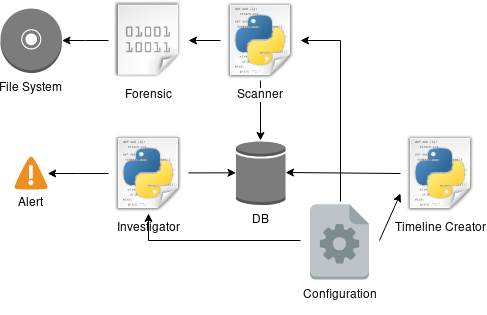
\includegraphics[width=8cm]{../img/Overview_FIDS.png}
  \centering
  \caption{Authenticator Data}
  \label{fig:authenticationMapping}
\end{figure}


\subsection{Scanner}
\label{sec:Scanner}

\subsection{Detection}
\label{sec:Detection}

\subsection{Configuration}
\label{sec:Configuration}

\subsubsection{Aide Configuration}
\label{sec:aide:config}

\subsection{Database}
\label{sec:Database}


\section{Application Flow}
\label{sec:flwo}


\section{Security}
\label{sec:Security}

\subsection{Limitations}
\label{sec:Limitations}

\subsection{Attack Scenarios}
\label{sec:attack_scenarios}


\chapter{Discussion}
\label{sec:Discussion}

\section{Future Work}
\label{sec:future:work}

\section{Attack Mittigations}
\label{sec:mittigations}

\chapter{Conclusion}
\label{sec:Conclusion}

\chapter{Journal}

\chapter{Implementation Details}

\section{Decisions}
\label{sec:decisions}

\subsection{Programming Language}
\label{sec:decisions:language}

\chapter{User Documentation}

\chapter{Project Management}

\section{Goal}
\label{apdx-sec:goal}
Before the start of the project the following main goal was defined:

Building of an \gls{hids} that detects unauthorized or unusual behaviour on the file system. Compared to traditional \gls{hids} file system integrity checking, it should scale with a lot of data and have the possibility to be used for investigation (retain historic data) built in from the start.

\subsection{Sub goals}

From this primary goal, the following sub goals were defined. 

\subsubsection{Scanning}
The system is capable of scanning the file system for certain properties. The search is done by leveraging the sleuthkit tools. Thus the system is capable of interpreting the results from sleuthkit. It will further analyze them and decide on what to do with the results. Especially importance is given to the finding of differences.

\subsubsection{Recording}
The system records all findings. Including new, changed and deleted files in comparison to an earlier point in time. This recording enables the use of investigation as the evolution of the data can be viewed at any time. This data can also be used for machine learning algorithms to detect anomalies that are out of the scope of this thesis. 

\subsubsection{Evaluation}
The system is capable of evaluating the results by applying predefined rules. Those rules can be adjusted by configuring the system.

It is thinkable that the system analyzes the recordings and makes decisions based on the historical behavior of the specific host and behavior from different similar hosts. This approach is not part of this thesis as it requires much historical data that is not present at the time of this thesis. 

\subsubsection{Alerting}
The system is capable of being run continuously. This capability enables it to find anomalies automatically. The system can report those anomalies by creating alerts. It allows configuration of these alerts.

\subsubsection{Scaling}
The run of the system on a big file system completes in an appropriate amount of time. This speed allows the finding of anomalies that appeared recently. Additionally, it allows the storing of more states of the system which results in a her probability of capturing short-lived anomalies for future investigations. 

\section{Workpackages}

From those goals the workpackages in table \ref{tab:workpackages} were defined. For a better overview they are assigned to categories. The categories are Architecture, Implementation, Validation and Administrative. Architecture is about defining how the system will look like and how it should work. Implementation is the effective implementation work for getting the system to run, this includes configuration and coding. Validation is about testing of the system. Administrative is everything that deals with project management and other workpackages that don't directly influence the system but need to be done.

The ID is a combination of the first letter of the category and a unique index. Administrative is shortened to D due to the conflict with Architecture.

The priority is a value of high, medium and low. 

The workpackages are chrononically ordered. Meaning they should be worked on in approximately the order that they are given. 

\begin{table}[h!]
  \begin{center}
    \caption{Workpackages}
    \label{tab:workpackages}
    \begin{tabular}{c|l|c|l}
      \textbf{ID} & \textbf{Short description} & \textbf{Prio} & \textbf{Category} \\
      \hline
      D00 & Setting up \LaTeX -document & h & Administrative \\
      D01 & Define workpackages and set deadlines & h & Administrative \\
			A00 & Research other \gls{hids} and the sleuthkit tools & h & Architecture \\
			A01 & Decide on a Programming Language & h & Architecture \\
			I00 & Setup the developer environment & h & Implementation \\
			I01 & Add the ability to scan the whole system using sleuthkit & h & Implementation \\
			A02 & Decide which database connectors should be used & h & Architecture \\
			I02 & Add one database connector & h & Implementation \\
			I03 & Implement a recording functionality & h & Implementation \\
			A03 & Decide how the rules should be defined & h & Architecture \\
			I04 & Add template rules and ability to parse them & h & Implementation \\
			I05 & Add functionality to parse output according to rules & h & Implementation \\
			V00 & Verify that the system runs on a big file system & h & Validation \\
			I06 & Add functionality of repeated scans & m & Implementation \\
			A04 & Define which alerting methods make sense & m & Architecture \\ 
			I07 & Add alerting functionality using one method & m & Implementation \\
			V01 & Verify the functionality of the software by changing the system & h & Validation \\
			V02 & Verify the functionality of the software by running it on an infected system & m & Validation \\
			V03 & Verify the alerting of the software by running it on an infectable system & m & Validation \\
			I08 & Add multiple database connectors to different systems & m & Implementation \\
			I09 & Add multiple alerting methods & m & Implementation \\
			A05 & Define how to protect system and configuration from tampering & l & Architecture \\
			I10 & Implement software hardening & l & Implementation \\
			D02 & Finish user documentation & m & Administrative \\
			D03 & Finish project documentation & h & Administrative \\ 
			D04 & Create project presentation & h & Administrative \\
			D05 & Create project poster & m & Administrative \\
			D06 & Create project video & l & Administrative \\
    \end{tabular}
  \end{center}
\end{table}

\section{Planning}

For the planning of this project the following milestones were created. Each coveres multiple workpackages. The mapping can be seen in table \ref{tab:milestones}. The milestones can also be seen in figure \ref{apdx-fig:milestones}. There they are displayed with an assumed and actual finish date.



\begin{table}[h!]
  \begin{center}
    \caption{Milestones}
    \label{tab:milestones}
    \begin{tabular}{c|l|c|l}
      \textbf{ID} & \textbf{Short description} & \textbf{Workpackages} \\
      \hline
			00 & Setup & D00, D01, A00, A01, I00 \\
			01 & Initial functionality & A02, I01, I02, I03 \\
			02 & Rules & A03, I04, I05, V00 \\
			03 & Alerting & A04, I06, I07 \\
			04 & Exhaustive testing & V01, V02, V03 \\
			05 & Usability & I08, I09, D02 \\
			06 & Software Hardening & A05, I10 \\
			07 & Presentation & D02, D03, D04, D05, D06 \\
    \end{tabular}
  \end{center}
\end{table}


\begin{figure}[H]
	\begin{ganttchart}[
		hgrid,
		vgrid,
		x unit=7mm,
		y unit chart=10mm,
		milestone label font = \footnotesize
	]{1}{17}
	\gantttitle{2019}{17}\\
	\gantttitlelist{1,...,17}{1}\\
	
	\ganttplannedmilestone{Setup}{4}
	\ganttactualmilestone{}{0}\\
	\ganttplannedmilestone{Initial functionality}{5}
	\ganttactualmilestone{}{0}\\
	\ganttplannedmilestone{Rules}{7}
	\ganttactualmilestone{}{0}\\
	\ganttplannedmilestone{Alerting}{8}
	\ganttactualmilestone{}{0}\\
	\ganttplannedmilestone{Exhaustive testing}{10}
	\ganttactualmilestone{}{0}\\
	\ganttplannedmilestone{Usability}{13}
	\ganttactualmilestone{}{0}\\
	\ganttplannedmilestone{Software Hardening}{15}
	\ganttactualmilestone{}{0}\\
	\ganttplannedmilestone{Presentation}{17}
	\ganttactualmilestone{}{0}
	\end{ganttchart}
	\caption{Milestones}
	\label{apdx-fig:milestones}
	\end{figure}

\section{Meetings}

\subsection{Template}

Hi Bruce,

Next Meeting:

Discussions:

Next Steps:

Julian


\newpage



\clearpage


\printglossaries

\clearpage

%% Print the bibibliography and add the section to the table of content
\printbibliography[heading=bibintoc]

%% Print the bibibliography and add the section to the table of content

\end{document}
